\documentclass[12pt]{article}
\usepackage{amsmath,amssymb}
\usepackage{geometry}
\geometry{margin=1in}
\usepackage{tikz}
\usetikzlibrary{decorations.pathmorphing,arrows.meta,calc}
\begin{document}

\begin{center}
\Large \textbf{Advanced Integrated Physics Problem Set — II (Ultra-Hard Extended Version)}
\end{center}

\bigskip

\textbf{Q1.}

A small bead of mass $m$ carrying charge $q$ is constrained to move without friction on a rigid circular hoop of radius $R$. The hoop is mounted vertically and rotates with constant angular speed $\omega$ about its vertical diameter passing through its center. A uniform magnetic field $ \vec B = B\hat z $ is present in space.

The position of the bead is described by angle $\theta$ measured from the lowest point of the hoop. Taking into account Coriolis effects in the rotating frame, magnetic Lorentz force, and constraint forces, determine the angular frequency of small oscillations about the stable equilibrium configuration.

\begin{center}
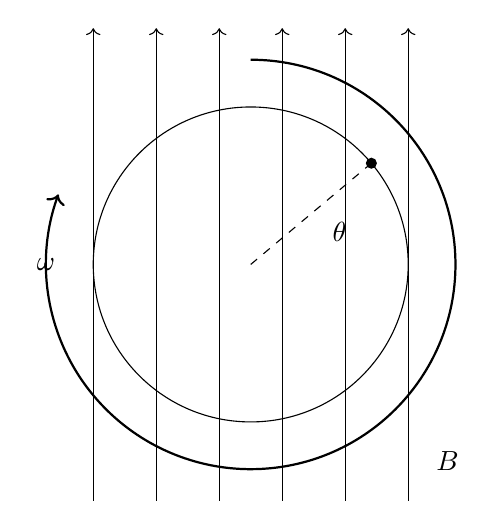
\begin{tikzpicture}[scale=1]

% Hoop
\draw (0,0) circle (2);

% Rotation circular arrow
\draw[->,thick] (0,2.6) arc[start angle=90,end angle=-200,radius=2.6];
\node at (-2.6,0){$\omega$};

% Magnetic field (vertical upward)
\foreach \x in {-2,-1.2,-0.4,0.4,1.2,2}
{
\draw[->] (\x,-3)--(\x,3);
}
\node at (2.5,-2.5){$B$};

% Bead
\fill (40:2) circle (2pt);

% Angle
\draw[dashed] (0,0)--(40:2);
\node at (20:1.2){$\theta$};

\end{tikzpicture}
\end{center}

\begin{enumerate}
\item[(A)] $\sqrt{\dfrac{g}{R}-\omega^2+\dfrac{qB\omega}{m}}$
\item[(B)] $\sqrt{\dfrac{g}{R}-\omega^2-\dfrac{qB\omega}{m}}$
\item[(C)] $\sqrt{\dfrac{g}{R}+\omega^2-\dfrac{qB\omega}{m}}$
\item[(D)] $\sqrt{\dfrac{g}{R}+\omega^2+\dfrac{qB\omega}{m}}$
\end{enumerate}

\bigskip

\textbf{Q2.}

A particle of mass $m$ moves under a central force field derived from the potential  
\[
U(r)= -\frac{k}{r} + \frac{\alpha}{2r^2},
\]
where $k>0$ and $\alpha$ may be positive or negative. The particle is in a circular orbit of radius $r_0$ corresponding to angular momentum $L$.

By analyzing the curvature of the effective potential and considering perturbations about $r_0$, determine the frequency of small radial oscillations. Carefully account for the contribution of both inverse and inverse-square potentials.

\begin{enumerate}
\item[(A)] $\sqrt{\dfrac{k}{mr_0^3}-\dfrac{3\alpha}{mr_0^4}}$
\item[(B)] $\sqrt{\dfrac{k}{mr_0^3}+\dfrac{3\alpha}{mr_0^4}}$
\item[(C)] $\sqrt{\dfrac{3k}{mr_0^3}-\dfrac{\alpha}{mr_0^4}}$
\item[(D)] $\sqrt{\dfrac{3k}{mr_0^3}+\dfrac{\alpha}{mr_0^4}}$
\end{enumerate}

\bigskip

\textbf{Q3.}

A block of mass $m$ is constrained to slide inside a smooth radial groove cut in a horizontal disc rotating with constant angular speed $\omega$. The block is connected to a vertical light spring of force constant $k$ whose other end is fixed at the center of the disc.

Assuming small oscillations about the equilibrium position and including the effect of centrifugal and Coriolis terms in the rotating frame, determine the frequency of small oscillations along the groove.

% Q3 Diagram
\begin{center}
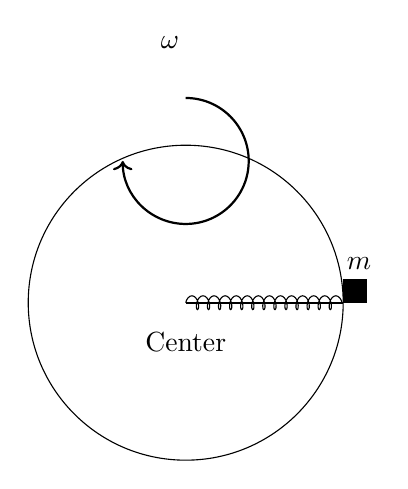
\begin{tikzpicture}[scale=1]
\draw (0,0) circle (2);
\draw[thick] (0,0)--(2,0);
\filldraw (2,0) rectangle (2.3,0.3);
\draw[decorate,decoration={coil,aspect=0.5,segment length=4pt}] (0,0)--(2,0);
\node at (0,-0.5){Center};
\node at (2.2,0.5){$m$};
\draw[->,thick] (0,2.6) arc[start angle=90,end angle=-180,radius=0.8];
\node at (-0.2,3.3){$\omega$};
\end{tikzpicture}
\end{center}

\begin{enumerate}
\item[(A)] $\sqrt{\dfrac{k}{m}-\omega^2}$
\item[(B)] $\sqrt{\dfrac{k}{m}-2\omega^2}$
\item[(C)] $\sqrt{\dfrac{k}{m}+\omega^2}$
\item[(D)] $\sqrt{\dfrac{k}{m}-3\omega^2}$
\end{enumerate}

\bigskip

\textbf{Q4.}

A conducting rod of length $L$ and mass $m$ is placed on two parallel conducting rails inclined at angle $\alpha$ to the horizontal. The rails are connected through a resistor $R$, and a uniform magnetic field $B$ acts perpendicular to the plane of the rails.

Starting from rest, the rod slides down due to gravity while an induced current produces a magnetic damping force. After sufficient time the rod reaches terminal velocity. Determine this terminal speed by balancing electromagnetic and mechanical power.

\begin{center}
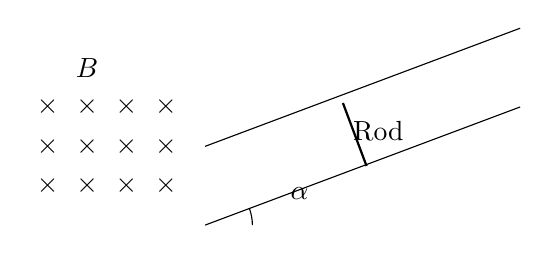
\begin{tikzpicture}[scale=1]

% Inclined rails
\draw (0,0)--(4,1.5);
\draw (0,1)--(4,2.5);

% Angle alpha
\draw (0.6,0) arc[start angle=0,end angle=21,radius=0.6];
\node at (1.2,0.4){$\alpha$};

% Rod perpendicular to rails
\draw[thick] (2.05,0.75)--(1.75,1.55);
\node at (2.2,1.2){Rod};

% Magnetic field into page
\foreach \x in {-0.5,-1,-1.5,-2}
{
\foreach \y in {0.5,1,1.5}
{
\node at (\x,\y){$\times$};
}
}
\node at (-1.5,2){$B$};

\end{tikzpicture}
\end{center}

\begin{enumerate}
\item[(A)] $\dfrac{mgR\sin\alpha}{B^2L^2}$
\item[(B)] $\dfrac{mgR\sin\alpha}{2B^2L^2}$
\item[(C)] $\dfrac{2mgR\sin\alpha}{B^2L^2}$
\item[(D)] $\dfrac{mgR\sin\alpha}{\pi B^2L^2}$
\end{enumerate}

\bigskip

\textbf{Q5.}

Two identical masses $m$ are connected by a light spring of force constant $k$ and are constrained to move on a smooth horizontal table. The entire system is observed from a frame rotating with constant angular speed $\omega$ about a vertical axis through the center of mass.

Considering small symmetric oscillations where both masses move equally and taking into account fictitious forces in the rotating frame, determine the normal mode frequency of this symmetric motion.

\begin{enumerate}
\item[(A)] $\sqrt{\dfrac{2k}{m}-\omega^2}$
\item[(B)] $\sqrt{\dfrac{2k}{m}-2\omega^2}$
\item[(C)] $\sqrt{\dfrac{k}{m}-\omega^2}$
\item[(D)] $\sqrt{\dfrac{k}{m}-2\omega^2}$
\end{enumerate}

\bigskip

\textbf{Q6.}

A parallel plate capacitor of plate area $A$ and separation $d$ is connected to a battery of constant voltage $V$. A dielectric slab of dielectric constant $\kappa$ is partially inserted between the plates and attached to a horizontal spring of stiffness $k$.

If the slab is slightly displaced from its equilibrium position, derive the restoring force using energy considerations and determine the frequency of small oscillations about equilibrium.

% Q6 Diagram
\begin{center}
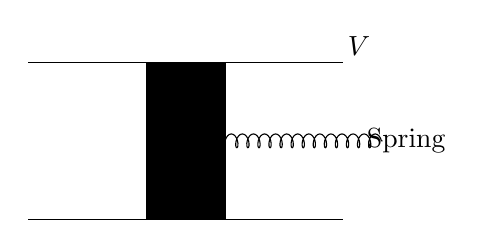
\begin{tikzpicture}[scale=1]
\draw (-2,1)--(2,1);
\draw (-2,-1)--(2,-1);
\filldraw (-0.5,-1) rectangle (0.5,1);
\node at (0,0){$\kappa$};
\draw[decorate,decoration={coil,aspect=0.5,segment length=4pt}] (0.5,0)--(2.5,0);
\node at (2.8,0){Spring};
\node at (2.2,1.2){$V$};
\end{tikzpicture}
\end{center}

\begin{enumerate}
\item[(A)] $\sqrt{\dfrac{k - \dfrac{\epsilon_0 A V^2 (\kappa -1)}{2d^3}}{m}}$
\item[(B)] $\sqrt{\dfrac{k - \dfrac{\epsilon_0 A V^2 (\kappa -1)}{d^3}}{m}}$
\item[(C)] $\sqrt{\dfrac{k + \dfrac{\epsilon_0 A V^2 (\kappa -1)}{2d^3}}{m}}$
\item[(D)] $\sqrt{\dfrac{k}{m}}$
\end{enumerate}

\bigskip

\textbf{Q7.}

A satellite of mass $m$ moves in a nearly circular orbit of radius $r$ around a planet of mass $M$. In addition to gravitational attraction, a small tangential drag force  
\[
F = -\epsilon \frac{GMm}{r^2}
\]
acts opposite to the velocity, where $\epsilon \ll 1$.

Using energy and angular momentum considerations, determine the fractional change in orbital radius after one complete revolution, retaining only first-order terms in $\epsilon$.

\begin{enumerate}
\item[(A)] $-\epsilon$
\item[(B)] $-\dfrac{\epsilon}{2}$
\item[(C)] $-2\epsilon$
\item[(D)] $-\dfrac{3\epsilon}{2}$
\end{enumerate}

\bigskip

\textbf{Q8.}

A charged bead moves on a fixed smooth helical wire of radius $R$ and pitch $p$. The axis of the helix is vertical and a uniform magnetic field $B$ acts vertically upward.

If the bead moves with constant speed along the helix, determine the condition for equilibrium by resolving gravitational and magnetic forces along the tangent to the helix.

\begin{center}
\begin{tikzpicture}[scale=1]

% Helix projection
\draw[domain=0:720,smooth,variable=\t]
plot ({1.2*cos(\t)}, {0.01*\t});
\fill ({1.2*cos(180)}, {0.01*180}) circle (2pt);



% Vertical magnetic field
\foreach \y in {0,0.8,1.6,2.4}
{
\draw[->] (-2,\y)--(-2,\y+0.5);
}
\node at (-2.3,3){$B$};

\node at (1.5,2.5){Helix};

\end{tikzpicture}
\end{center}

\begin{enumerate}
\item[(A)] $mg=qBv$
\item[(B)] $mgp=2\pi qBRv$
\item[(C)] $mgR=qBvp$
\item[(D)] $mgp=qBRv$
\end{enumerate}

\bigskip

\textbf{Q9.}

A particle of mass $m$ moves in a one-dimensional potential  
\[
U(r) = \frac12 kr^2 + \beta r^4.
\]
The particle executes small oscillations about a stable equilibrium position $r_0$ corresponding to minimum energy.

By expanding the potential about $r_0$ up to quadratic order and determining the curvature of the potential well, find the frequency of small oscillations.

\begin{enumerate}
\item[(A)] $\sqrt{\dfrac{k}{m}+\dfrac{12\beta r_0^2}{m}}$
\item[(B)] $\sqrt{\dfrac{k}{m}+\dfrac{6\beta r_0^2}{m}}$
\item[(C)] $\sqrt{\dfrac{k}{m}+\dfrac{3\beta r_0^2}{m}}$
\item[(D)] $\sqrt{\dfrac{k}{m}+\dfrac{2\beta r_0^2}{m}}$
\end{enumerate}

\bigskip

\textbf{Q10.}

An LC circuit has one plate of the capacitor mounted on a movable platform of mass $m$ attached to a spring of stiffness $k$. The capacitor carries charge $Q$ and has instantaneous separation $d$.

Considering coupling between electrical and mechanical degrees of freedom and linearizing the equations about equilibrium, determine the lower normal mode frequency of the system.

\begin{center}
\begin{tikzpicture}[scale=1]

% Fixed plate
\draw (-2,1)--(-2,-1);

% Movable plate
\draw (0,1)--(0,-1);

% Spring attached to movable plate
\draw[decorate,decoration={coil,aspect=0.5,segment length=4pt}] 
(0,0)--(2,0);
\node at (2.4,0){$k$};

% Inductor symbol
\draw (-3,0.6) to[out=0,in=180] (-2.5,0.6)
      to[out=0,in=180] (-2,0.6);

\node at (-1,1.3){$Q$};

\end{tikzpicture}
\end{center}

\begin{enumerate}
\item[(A)] $\sqrt{\dfrac{k}{m}}$
\item[(B)] $\sqrt{\dfrac{k}{m}-\dfrac{Q^2}{mC^2d^2}}$
\item[(C)] $\sqrt{\dfrac{k}{m}+\dfrac{Q^2}{mC^2d^2}}$
\item[(D)] $\sqrt{\dfrac{k}{m}-\dfrac{2Q^2}{mC^2d^2}}$
\end{enumerate}

\bigskip

\textbf{Q11.}

A bead slides without friction on a smooth cycloidal track whose plane rotates about a vertical axis passing through its cusp with constant angular speed $\omega$. The cycloid has generating circle radius $a$.

Assuming small oscillations about the lowest point and including the effect of centrifugal potential, determine the modified oscillation frequency.

% Q11 Diagram
\begin{center}
\begin{tikzpicture}[scale=1]
\draw[domain=0:360,smooth,variable=\t]
plot ({0.01745*\t - sin(\t)}, {1 - cos(\t)});
\fill ({180/57.3 - sin(180)}, {1 - cos(180)}) circle (2pt);
% Proper rotation arrow
\draw[->,thick] (-1,-1.5) arc[start angle=180,end angle=-180,radius=0.8];
\node at (-1,-2.6){$\omega$};
\end{tikzpicture}
\end{center}

\begin{enumerate}
\item[(A)] $\sqrt{\dfrac{g}{4a}-\omega^2}$
\item[(B)] $\sqrt{\dfrac{g}{4a}-2\omega^2}$
\item[(C)] $\sqrt{\dfrac{g}{4a}+\omega^2}$
\item[(D)] $\sqrt{\dfrac{g}{4a}-3\omega^2}$
\end{enumerate}

\bigskip

\textbf{Q12.}

A rigid rod of length $L$ and moment of inertia $I$ has charges $+q$ and $-q$ fixed at its ends. The rod is free to rotate in a plane perpendicular to uniform electric field $E$ while a uniform magnetic field $B$ is applied perpendicular to the plane.

Considering torque contributions due to electric forces and motional emf effects, determine the angular frequency of small oscillations about equilibrium orientation.

\begin{center}
\begin{tikzpicture}[scale=1]

\draw[thick] (-2,0)--(2,0);

\fill (-2,0) circle (2pt);
\fill (2,0) circle (2pt);

\node at (-2,0.3){$+q$};
\node at (2,0.3){$-q$};

% Electric field
\draw[->] (0,1)--(2,1);
\node at (2.3,1){$E$};

% Magnetic field into page
\foreach \x in {-1,-0.5,0,0.5,1}
{
\node at (\x,-1){$\times$};
}
\node at (1.5,-1.3){$B$};

\end{tikzpicture}
\end{center}

\begin{enumerate}
\item[(A)] $\sqrt{\dfrac{qEL}{I}}$
\item[(B)] $\sqrt{\dfrac{qEL}{2I}}$
\item[(C)] $\sqrt{\dfrac{qEL}{I}+\dfrac{qBL\omega}{I}}$
\item[(D)] $\sqrt{\dfrac{qEL}{2I}-\dfrac{qBL\omega}{I}}$
\end{enumerate}

\bigskip

\textbf{Q13.}

A particle moves under the effective potential  
\[
U = -\frac{GMm}{r} + \frac{L^2}{2mr^2} + \frac12 m\omega^2 r^2,
\]
which includes gravitational attraction, centrifugal barrier due to angular momentum $L$, and an additional harmonic confinement.

Determine the condition for equilibrium radius and identify the correct expression governing the stable orbit by solving $dU/dr = 0$.

\begin{enumerate}
\item[(A)] $\left(\dfrac{GM}{\omega^2}\right)^{1/3}$
\item[(B)] $\left(\dfrac{L^2}{m^2\omega^2}\right)^{1/4}$
\item[(C)] solution of $GM=\omega^2r^3-\dfrac{L^2}{mr}$
\item[(D)] $\left(\dfrac{2GM}{\omega^2}\right)^{1/3}$
\end{enumerate}

\bigskip

\textbf{Q14.}

A thin ring of radius $R$ rolls without slipping inside a vertical circular hoop which rotates about its vertical diameter with constant angular speed $\omega$. The motion is constrained such that the ring always remains in contact with the hoop.

Analyze stability of the equilibrium at the highest point by considering effective potential in the rotating frame and determine the condition on $\omega$ for stability.

% Q14 Diagram
\begin{center}
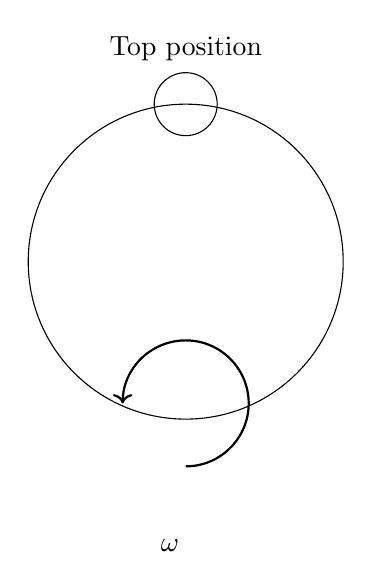
\begin{tikzpicture}[scale=1]
\draw (0,0) circle (2);
\draw (0,2) circle (0.4);
\node at (0,2.7){Top position};
\draw[->,thick] (0,-2.6) arc[start angle=-90,end angle=180,radius=0.8];
\node at (-0.2,-3.6){$\omega$};

\end{tikzpicture}
\end{center}

\begin{enumerate}
\item[(A)] $\omega^2>\dfrac{g}{R}$
\item[(B)] $\omega^2>\dfrac{2g}{R}$
\item[(C)] $\omega^2>\dfrac{3g}{R}$
\item[(D)] $\omega^2>\dfrac{4g}{R}$
\end{enumerate}

\bigskip

\textbf{Q15.}

A particle moves in a rotating frame with angular speed $\omega$ under the combined influence of gravitational attraction due to a central mass $M$ and centrifugal potential of the rotating frame.

By constructing the effective potential and minimizing it with respect to radius, determine the stable circular orbit radius and discuss conditions for stability against small perturbations.

\begin{enumerate}
\item[(A)] $\left(\dfrac{GM}{\omega^2}\right)^{1/3}$
\item[(B)] $\left(\dfrac{2GM}{\omega^2}\right)^{1/3}$
\item[(C)] $\left(\dfrac{GM}{2\omega^2}\right)^{1/3}$
\item[(D)] $\left(\dfrac{3GM}{\omega^2}\right)^{1/3}$
\end{enumerate}

\end{document}